\section{PTDL volume integrator}
\label{section:ptdl_implement}
As described it the theoretical introduction to the volumetric path tracing integrators
\ref{section:udpt}, the Next Event Estimation can be considered as a valuable improvement of the
brute force unidirectional path tracing in certain scenarios. Path Tracing Direct Light (\gls{PTDL})
integrator was implemented as an independent solution for light simulation in participating media in
this work. Let us take a closer look at the implementation details of this technique.

After the a ray is hitting the subsurface scattering object, the algorithm starts the construction
of the path similar to that for brute force volumetric path tracing. At each vertex position
$\mathbf{x}_i$ of the path the location of the next vertex is constructed as
\[
\mathbf{x}_{i}=\mathbf{x}_{i-1}+d_i\vec{\omega_i}
\]
where symbols in \textbf{bold} represent the vectors of the position, and $\vec{\omega}_i$ stands
for direction vector.

The distance $d_i$ to the next vertex $\mathbf{x}_{i}$ (i.e. the length of the random walk
step) is sampled according to the Beer--Lambert law, with $\xi$ as a uniform distributed random
variable:
\begin{align}
\label{eq:beers_lambert_sampling}
d_i = \frac{ln(\xi)}{\sigma_s}
\end{align}
Attenuation coefficient is not taken into account at this step an will be considered later while
integrating the light contribution.

\begin{figure}[h]
    \centering
    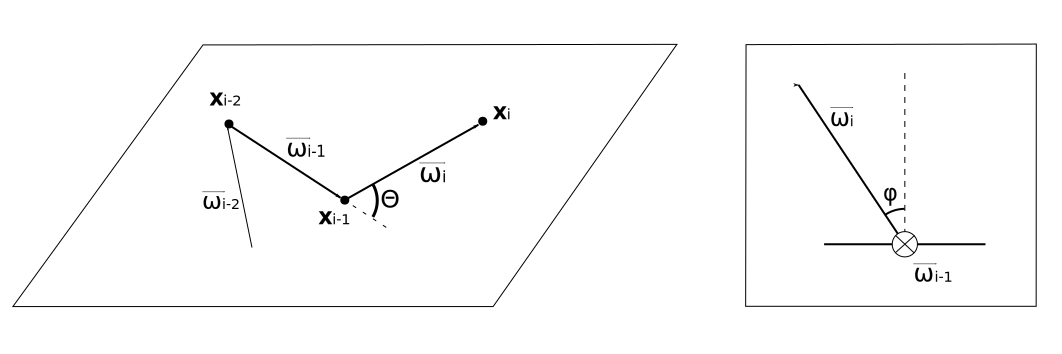
\includegraphics[width=0.85\textwidth]{imgs/schemes/omega}
    \caption{Polar and azimuthal angles for random walk step direction}
    \label{fig:omega}
\end{figure}

The direction $\vec{\omega}_i$ to the next vertex is chosen according to the sampling of the
phase function. In the simplest case of isotropic media, $\vec{\omega}_i$ has uniform distribution
around the sphere, independent of the previous step direction.
But in the case of anisotropic media while using Henyey-Greenstein phase function 
\ref{section:phasefunction}, the azimuthal angle $\varphi_i$ is sampled uniformly and the polar
angle $\Theta_i$ is according to Henyey-Greenstein function:
\[
\varphi_i(\xi)=2\pi\cdot\xi
\]
\begin{equation}
\label{eq:hg_sampling}
\cos{\Theta_i}(g, \xi) = \frac{1+g^2-(\frac{1-g^2}{1-g+2g\xi})^2}{2g} 
\end{equation}

Note, that random variable $\xi$ have to be generated each time independently for $d_i$, $\varphi_i$
and $\Theta_i$. The direction vector $\omega_i$ is calculated as shown on the figure \ref{fig:omega}
on the basis of the direction of the previous step $\omega_{i-1}$. The $\cos{\Theta_i}$ is also
equal to the dot product between the current and the previous steps directions
$\vec{\omega}_i\cdot\vec{\omega}_{i-1}$.

At each step after the direction and the distance to the next vertex is computed the intersection
test have to be performed to determine if the next vertex is located inside the current object or
not.
This is done by tracing of the regular ray in the computed direction $\vec{\omega}_i$ from the
previous vertex position $x_{i-1}$. The example of path construction is given on the figure
\ref{fig:path_ptdl}
\begin{figure}[h]
    \centering
    \includegraphics[width=0.6\textwidth]{imgs/schemes/path_ptdl}
    \caption{Path construction and direct light sampling}
    \label{fig:path_ptdl}
\end{figure}

If the next vertex is located inside the media, the direct light sampling (visibility
test of the light) step is preformed.
It is made by casting the \emph{Shadow ray} in the direction of the light source. Together with
the regular shadow weight contribution $s_i$, the distance $l_i$ from the current vertex position to
the object's closest surface location along the shadow ray have to be found (see figure
\ref{fig:path_ptdl}). $l_i$ is needed to account for the attenuation and out-scattering of the
light on the way from surface to the current vertex.

The outgoing (exitant) radiance at current vertex $L_o(\mathbf{x}_i, -\vec{\omega}_i)$ in the
direction to the previous vertex of the path is computed as the following sum:
\begin{align*}
L_o(\mathbf{x}_i, -\vec{\omega}_i) = &\phantom{\mid{}}
\underbrace{L_{o}(\mathbf{x}_{i+1}, -\vec{\omega}_{i+1})\cdot e^{-\sigma_a d_{i+1}}}_\text{incoming
 radiance from next vertex}+\\
& \phantom{\mid{}} +\underbrace{L_i(\mathbf{x}_i,-\vec{\omega}_{DL})}_\text{direct lighting
 estimation} \cdot \underbrace{\frac{1}{\text{pdf}(\vec{\omega}_{DL})}}_\text{phase function
 sampling probability} \cdot
\underbrace{e^{(\sigma_a+\sigma_s) l_i}}_\text{out scattering and attenuation}
\end{align*}

Note that the first term is multiplied by the attenuation decay only. No scattering coefficient is
involved there, because the next vertex of the path is computed stochastically by sampling
Beers-Lambert law as stated in equation \ref{eq:beers_lambert_sampling}.

But the attenuation of the direct light from the light source have to be computed with both
scattering and attenuation coefficients. The deterministic choice of the light path from the vertex
to the light also demands to multiply the incoming radiance by the inverse of the probability
density function of choosing this particular direction. This is the outcome of the Monte Carlo
integration as described in theoretical chapter \ref{Monte-Carlo}

The probability density of Henyey-Greenstein phase function is: 
\begin{align}
\label{eq:hg_pdf}
pdf(\cos{\Theta}) = \frac{1}{4\pi}\cdot\frac{1-g^2}{1+g^2-2g(\cos{\Theta})^{3/2}}
\end{align}
which is the source of the above mentioned sampling form \ref{eq:hg_sampling}

There is an approximation of the \ref{eq:hg_pdf} described in \cite{CGF:CGFCGF123_0201},

\[
pdf_{schlick}(\cos{\Theta}) = \frac{1}{4\pi}\frac{1-k^2}{(1-k\cos{\Theta})^2}
\]
with coefficient chosen as $k=1.55g-0.55g^3$ \cite[p.~586]{pharr2010physically}. The corresponding
sampling of the $\Theta$ have to be used while using this approximation instead of
\ref{eq:hg_sampling}

The direct light sampling is performed each time after the vertex of the path is generated. In case
if the new vertex is located outside of the object, the volumetric path tracing is terminated. This
is the distinct difference between \gls{PTDL} and classic volumetric path tracing. In the latter
case, only the lighting contribution at the last vertex o the path at the at the object
boundary would be computed and added to the contribution of the current path with respective
attenuation weight.

\subsection{Validation of the correctness of PTDL volume integrator}
After implementing the light integrator with direct light sampling at each step of a random walk
inside the media, we had to make sure that it is correct and converges to the same result as brute
force Monte Carlo volumetric path tracer.

As a first validation test we need to check if the integrator conserves energy and does not produce
brighter or darker results over the whole scene. Similar to the scene described in the previous
section \ref{section:numerical}, we use a simple object with subsurface material without attenuation
in absolutely white spherical environment. The idea is, that if no energy is added or taken from the
light source during the light simulation inside the media, the object should converge to absolutely
white appearance. The experiments with different values of the scattering coefficient $\sigma_s$
showed that the PTDL integrator passes this fast and simple test.

\begin{figure}
    \centering
    \begin{subfigure}{0.3\textwidth}
        \includegraphics[width=\textwidth]{imgs/renders/cube_area_ptdl}
        \caption{Original output}
    \end{subfigure}
    \quad
    \begin{subfigure}{0.3\textwidth}
        \includegraphics[width=\textwidth]{imgs/renders/cube_area_path_heat}
        \caption{Path tracing heat map}
    \end{subfigure}
    \begin{subfigure}{0.3\textwidth}
        \includegraphics[width=\textwidth]{imgs/renders/cube_area_ptdl_heat}
        \caption{PTDL heat map}
    \end{subfigure}
    \caption{Comparison of the same scene using different volumetric integrators,
    $\sigma_a=1mm^{-1}$, $\sigma_s=10mm^{-1}$ with the size of the cube 10x10x10mm}
    \label{fig:cube_area_compare}
\end{figure}

The next step for validation is to check the radiance distribution produced by the PTDL for
different kinds of light sources. We decided to test scenes with Image Based HDR lights and area
geometric lights of arbitrary shape. The special cases of analytic light sources such
as infinitesimal point lights and directional lights are naturally supported. But there is no way to
check the consistency because of the inherent inability of the brute force Monte Carlo path tracing
integrator to produce the reference images for such virtual lights. For these cases with made a
comparisons with independent implementation of the hybrid volumetric path tracer in Mitsuba renderer
\cite{Mitsuba}.

All the tests showed that the PTDL integrator produces the same output as the corresponding
reference. One of the test results are shown at the figure \ref{fig:cube_area_compare}

\subsection{Performance of PTDL}
The main practical advantage of the PTDL integrator over the brute force is the efficient sampling
of small and intense light sources or the IBL lights with the high frequency component like bright
sun.

Even taking into account the limitations of the current implementation (such as inability to
correctly reconstruct the path with refractive boundaries) the PTDL may show much better convergence
rate for particular scenes than classic volumetric path tracer.

\begin{figure}[h]
    \centering
    \begin{subfigure}{\textwidth}
        \includegraphics[width=\textwidth]{imgs/renders/spheres_path}
        \caption{Path tracing, 5s render time, 60 samples per pixel}
        \label{fig:spheres_path}
    \end{subfigure}
    \begin{subfigure}{\textwidth}
        \includegraphics[width=\textwidth]{imgs/renders/spheres_ptdl}
        \caption{Next event estimation, 5s render time, 20 samples per pixel}
        \label{fig:spheres_ptdl}
    \end{subfigure}
\end{figure}

To compare the variance of the estimations for different sizes of the light sources, we build
an equal time comparison as shown on the figures \ref{fig:spheres_path} and \ref{fig:spheres_ptdl}.
At the bottom row of each image we can see the tested objects with the same SSS materials. The
geometric light sources of various sizes contribute only to the illumination of the corresponding
object directly below each of them. The values of luminous flux of the light sources are equal. That
is the integral radiant flux of the light source is the same regardless of the total area.

We can clearly see the noticeable difference in the distribution of the noise for the integrators of
both types, depending on the light source size. The path tracer outperform PTDL for the case of the
large light source on the right. But in case of small light, the PTDL almost instantly produce the
result with the moderate amount of noise.

This are the expected performance results if we consider how both integrators work. In
the case of the large light scenario or uniform environment light, every, or almost every path from
the volume will contribute to the final result with high weight which will result in low variance.
But there is a little chance that the random ray outgoing from the object of the path tracer will
hit the small light source. In contrast, the direct lighting sampling at each vertex of the path of
the PTDL integrator makes sure that each, even small or virtual light is taken into account during
accumulation of the final result. Unfortunately, many visibility tests make traversing of each path
of the PTDL more expensive to compute.

These advantages and disadvantages of both sampling types are well described in the literature for
the cases of BSDF or light sampling during Global Illumination integration
\cite{Veach:1998:RMC:927297}, \cite{pharr2010physically}.
As a result, to employ the advantages of each method and build a robust integrator capable of rendering
both corner cases, it is necessary to combine them using Multiple Importance Sampling.

